%\documentclass[english, times, mirror]{revdetua}
% use this if you're writing in portuguese:
\documentclass[portuguese, times, mirror]{revdetua}

\usepackage[utf8]{inputenc}
\usepackage{graphicx}
\usepackage{hyperref}

\usepackage{amsmath}
\usepackage{mathtools}

\usepackage{caption}
\usepackage{listings}
\usepackage{color}

\definecolor{dkgreen}{rgb}{0,0.6,0}
\definecolor{gray}{rgb}{0.5,0.5,0.5}
\definecolor{mauve}{rgb}{0.58,0,0.82}

\lstset{frame=tb,
  language=Java,    
  aboveskip=3mm,
  belowskip=3mm,
  showstringspaces=false,
  columns=flexible,
  basicstyle={\small\ttfamily},
  numbers=none,
  numberstyle=\tiny\color{gray},
  keywordstyle=\color{blue},
  commentstyle=\color{dkgreen},
  stringstyle=\color{mauve},
  breaklines=true,
  breakatwhitespace=true,
  tabsize=3
}

\usepackage{tikz}
\usepackage{pgfplots}

% correct bad hyphenation here
\hyphenation{op-tical net-works semi-conduc-tor}

\begin{document}

\Header{1}{5}{Outubro}{2016}{1}
% Note: the month must be in Portuguese

\title{Visão por Computador 2016-17, Guia Prático N.º 7}
\author{Rui Oliveira, Tomás Rodrigues\\ DETI, Universidade de Aveiro \\ Aveiro, Portugal \\ \{ruipedrooliveira, tomasrodrigues\}@ua.pt}
% you should be able to use the \and keyword, but the deti format doesn't like it, for some reason
\maketitle

\begin{resumo}


Pretende-se através deste relatório expor sob forma escrita, o nosso desempenho e objetivos alcançados na aula prática n.º7 da unidade curricular de Visão por Computador do Mestrado Integrado de Engenharia de Computadores e Telemática.

Neste relatório pretenderemos explicar as soluções por nós encontradas para a resolução dos diferentes problemas propostos.


\end{resumo} 

\begin{palavraschave} %
visão, computador, imagem digital, stereo calibration, opencv, c++, 
 \end{palavraschave} %




\section{Repositório: código fonte}


Todas as soluções dos problemas propostos estão disponível através do seguinte repositório (gitHub) criado para o efeito. \\

\href{http://github.com/toomyy94/CV1617-68779-68129}{http://github.com/toomyy94/CV1617-68779-68129}
\\


A resolução dos problemas do presente guia encontram-se na pasta aula7. Para a resolução dos exercícios não foi usado nenhum IDE. Para a compilação do código fonte foi usada uma makefile. 



\section{Problemas propostos}



\subsection{Problema \#1 - \textit{Disparity map}}

\subsubsection{Enunciado}
\textit{Recover the code from the exercise on image rectification (exercise 5 in last lecture - in alternative  you might use the available code in reconstruct.cpp). Use the class StereoBM and the function that implements a block matching techniques (template matching will be explored later within this Computer Vision course) to find correspondences over two rectified stereo images. Use the parameters specified as follow since we will not enter in details of these functions.}


\subsubsection{Resolução e principais conclusões}

Para a resolução deste exercício foram seguidos os seguintes passos: 

\begin{enumerate}
    \item Ler parâmetros do ficheiro \texttt{stereoParams.xml} produzido na aula 6
    \item Ler imagens stereovision cedidas - imagem da esquerda e direita
    \item Aplicar métodos \texttt{stereoRectify} aos parâmetros intrinsics1, intrinsics2 , intrinsics1 e intrinsics2 com o objetivo de obter os parâmetros de rotação, translação...
    \item Aplicar método \texttt{initUndistortRectifyMap} para obter variáveis \texttt{map1x}, \texttt{map1y}, \texttt{map2x} e \texttt{map2y} 
    \item Aplicar \texttt{cv::cvtColor(imagel, gray\_imagel , CV\_RGB2GRAY);}
    \item Aplicar \texttt{cv::remap(gray\_imagel, remap\_imgl, map1x, map1y,cv::INTER\_LINEAR);}
    \item Aplicar os dois item anteriores à imagem da direita.
    \item Aplicar o excerto de código disponível no enunciado desta aula.
    \item Visualizar o resultado da disparidade. 

    
\end{enumerate}

O resultado obtidos pode ser observado na seguinte figura. 

\begin{figure}[ht!]
\centering
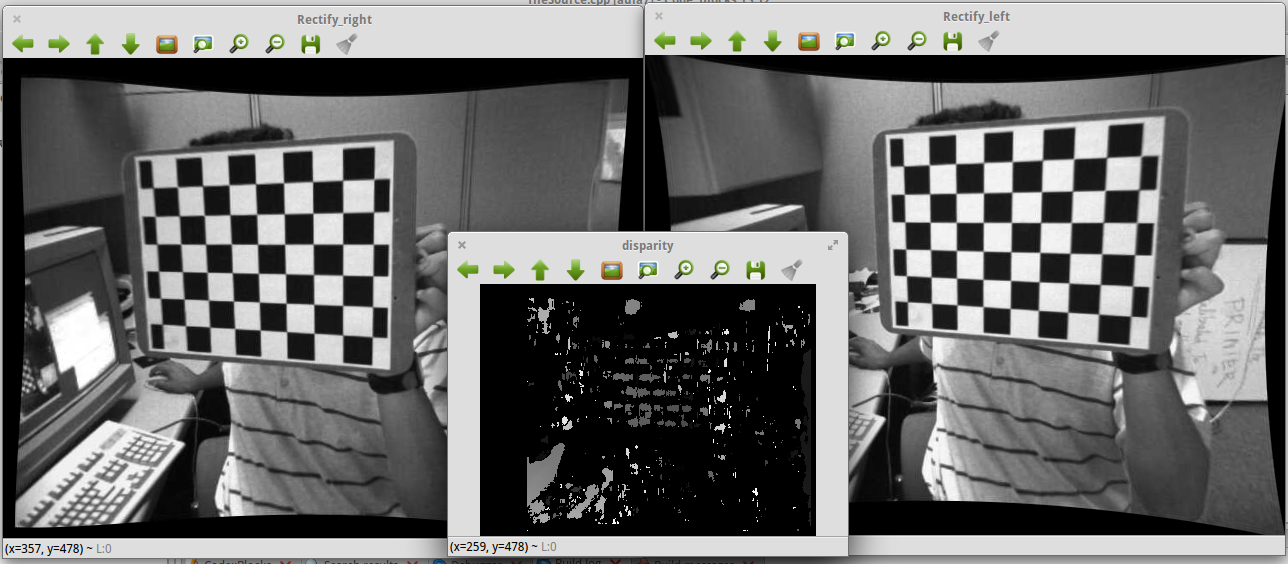
\includegraphics[width=70mm]{img/ex1.png}
\caption{Resultado obtido após exercício 1}
\end{figure}


%%%%%%%%%%%%%%%%%%%%%%%%%%%%%%%%%%%%%%%%%%%%%%%%%%%%%%%%%%%%%%5
%%%%%%%%%%%%%%%%%%%%%%%%%%%%%%%%%%%%%%%%%%%%%%%%%%%%%%%%%%%%%%%

\subsection{Problema \#2 - \textit{3D Reconstruction}}

\subsubsection{Enunciado}
\textit{Use the function cvReprojectImageTo3D to compute the 3D coordinates of the pixels in the disparity 
map. The parameters of cvReprojectImageTo3D are the disparity map (disp in previous exercise), and the
matrix Q given by the function cvStereoRectify. Save the 3D coordinates in an xml file using the 
function FileStorage}


\subsubsection{Resolução e principais conclusões}

Este exercício resultou de uma continuação do exercício anterior. No final desse, foi invocada a função \texttt{reprojectImageTo3D} com a variável resultante da função \texttt{imgDisparity16S.convertTo()}. Posteriormente foi gerado um ficheiro XML resultante da matrix \texttt{points3d}.  


\begin{lstlisting}[caption=Aplicação da função reprojectImageTo3D e criação do ficheiro XML ,label=code:C]
Mat points3d;
reprojectImageTo3D(imgDisparity16S, points3d, Q);

cv::FileStorage fs2("../points3d.xml", cv::FileStorage::WRITE);
if (!fs.isOpened()) {
    std::cout << "Failed to open stereoParams.xml" << std::endl;
    return 1;
}
fs2 << "points" << points3d;
fs2.release();

\end{lstlisting}



\begin{lstlisting}[caption=points3d.xml ,label=code:xml]

<?xml version="1.0"?>
<opencv_storage>
<points type_id="opencv-matrix">
  <rows>480</rows>
  <cols>640</cols>
  <dt>"3f"</dt>
  <data>
    6.71058960e+01 5.05488701e+01 -9.15517426e+01 6.68978424e+01
    5.05488701e+01 -9.15517426e+01 6.66897888e+01 5.05488701e+01
    -9.15517426e+01 6.64817276e+01 5.05488701e+01 -9.15517426e+01
    6.62736740e+01 5.05488701e+01 -9.15517426e+01 6.60656128e+01
    5.05488701e+01 -9.15517426e+01 6.58575592e+01 5.05488701e+01
    -9.15517426e+01 6.56495056e+01 5.05488701e+01 -9.15517426e+01
...
\end{lstlisting}




%%%%%%%%%%%%%%%%%%%%%%%%%%%%%%%%%%%%%%%%%%%%%%%%%%%%%%%%%%%%%%5
%%%%%%%%%%%%%%%%%%%%%%%%%%%%%%%%%%%%%%%%%%%%%%%%%%%%%%%%%%%%%%%


\subsection{Problema \#3 - \textit{Visualization of point cloud in pcl}}

\subsubsection{Enunciado}
\textit{Modify the source code viewcloud.cpp to read the 3D points of the file you have saved in the
previous section and visualize the results of the 3D reconstruction. 
Assignment to the pointCloud (cloud in the example below) can be performed using the following
code (or similar): }

\begin{lstlisting}[caption=Excerto de código (enunciado),label=code:C]
int p=0;
for (int i=0;i< (*cloud).height; i++)
for (int j=0;j< (*cloud).width; j++)
{
(*cloud).points[p].x = pos3D.at<cv::Vec3f>(i,j)[0];
(*cloud).points[p].y = pos3D.at<cv::Vec3f>(i,j)[1];
(*cloud).points[p].z = pos3D.at<cv::Vec3f>(i,j)[2];
p++;
} 
\end{lstlisting}

\textit{Visualize the 3 points and add any filtering necessary to avoid visualization of not well reconstructed 3d Points.}


\subsubsection{Resolução e principais conclusões}

Começámos por ler o ficheiro \texttt{points3d.xml} resultante do exercício anterior. O resultado da leitura foi colocado na variavel \texttt{pos3D}. Posteriormente, as variáveis \texttt{width}, \texttt{height} e  \texttt{is\_dense} foram inicializadas da seguinte forma: 

\begin{lstlisting}[caption=Inicialização de variáveis ,label=code:C]
(*cloud).width = pos3D.size().width;
(*cloud).height = pos3D.size().height;
(*cloud).is_dense = false;
(*cloud).points.resize((*cloud).width * (*cloud).height);
\end{lstlisting}


Seguidamente, foi utilizado o excerto de código que consta no enunciado deste exercício. 

\begin{figure}[ht!]
\centering
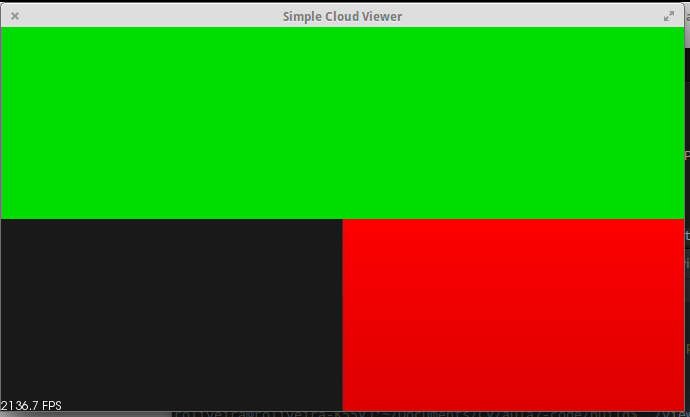
\includegraphics[width=70mm]{img/ex3_1.png}
\caption{Resultado obtido após exercício 3}
\end{figure}


\begin{figure}[ht!]
\centering
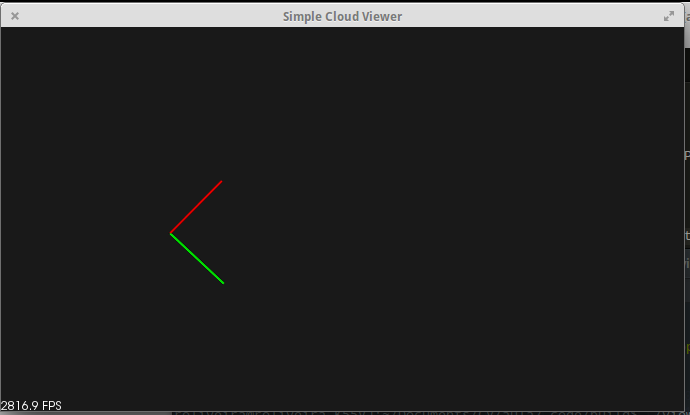
\includegraphics[width=70mm]{img/ex3_2.png}
\caption{Resultado obtido após exercício 3}
\end{figure}

%%%%%%%%%%%%%%%%%%%%%%%%%%%%%%%%%%%%%%%%%%%%%%%%%%%%%%%%%%%%%%5
%%%%%%%%%%%%%%%%%%%%%%%%%%%%%%%%%%%%%%%%%%%%%%%%%%%%%%%%%%%%%%%


\subsection{Problema \#4 - \textit{PCD (point cloud data) 3D format}}

\subsubsection{Enunciado}
\textit{Modify the source code viewcloud.cpp to read and visualize the two provided kinect images 
filt\_office1.pcd and filt\_office2.pcd The Point Cloud Data file format (PCD) used is the 3D file
format from PCL and can be written and read directly using the PCL functions loadPCDfile and 
savePCDFileASCII. }


\subsubsection{Resolução e principais conclusões}

Para a resolução deste exercício foram criados dois variáveis do tipo \texttt{PointCloud<PointXYZRGB>::Ptr} : \texttt{cloud1} e \texttt{cloud2}. 
Posteriormente foram carregados os ficheiros \texttt{filt\_office1.pcd} e \texttt{filt\_office2.pcd} respetivamente para as variáveis \texttt{cloud1} e \texttt{cloud2}. Finalmente, foi usado o método \texttt{showCloud()} para visualização. O resultado obtido pode ser observado nas seguintes imagens. 

\begin{figure}[ht!]
\centering
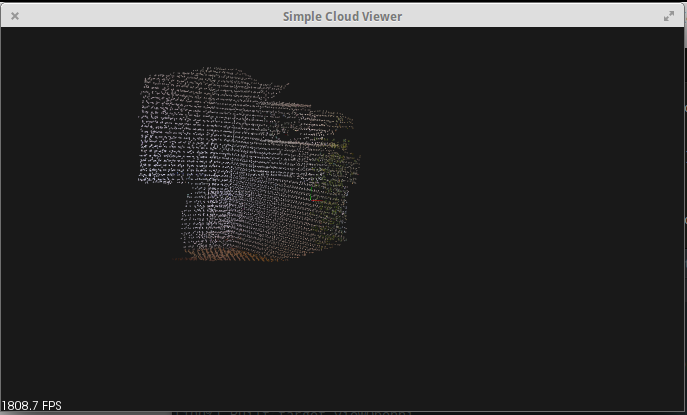
\includegraphics[width=70mm]{img/ex4_1.png}
\caption{Resultado obtido após exercício 4}
\end{figure}


\begin{figure}[ht!]
\centering
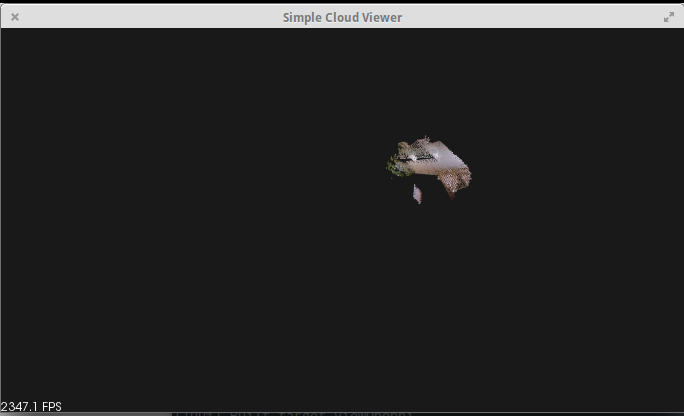
\includegraphics[width=70mm]{img/ex4_2.png}
\caption{Resultado obtido após exercício 4}
\end{figure}


\begin{figure}[ht!]
\centering
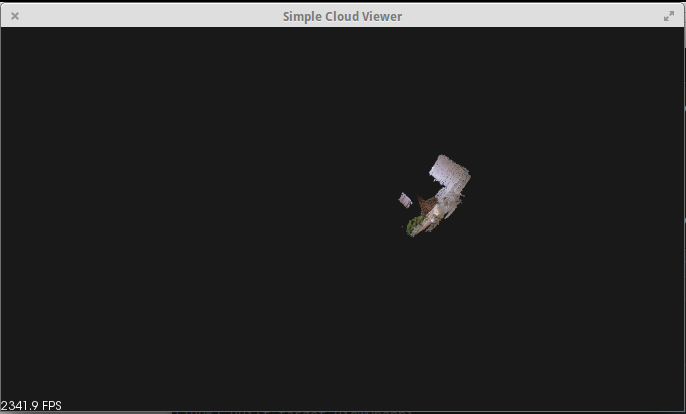
\includegraphics[width=70mm]{img/ex4_3.png}
\caption{Resultado obtido após exercício 4}
\end{figure}


%%%%%%%%%%%%%%%%%%%%%%%%%%%%%%%%%%%%%%%%%%%%%%%%%%%%%%%%%%%%%%5
%%%%%%%%%%%%%%%%%%%%%%%%%%%%%%%%%%%%%%%%%%%%%%%%%%%%%%%%%%%%%%%

\subsection{Problema \#5 - \textit{ICP alignment}}

\subsubsection{Enunciado}
\textit{Use the pcl::IterativeClosestPoint function to align the given down sampled cloud of points. Note 
that the values of the termination criteria are very sensitive and should be adapted for each case.
Normally an initial rough registration should also be provided to avoid bad registration However in this
case, and given the proximity of the provided depth images this should not be necessary. }


\subsubsection{Resolução e principais conclusões}

Para a resolução deste exercício foi utilizado o ficheiro \texttt{viewFreenect.cpp} disponibilizado. A linha \texttt{change\_color(aligned\_cloud,0,0,255);} foi substituída pelo excerto de código que a seguir se apresenta. 

\newpage

\begin{lstlisting}[caption=colors cloudAligned red for viewing purposes,label=code:C]
int p = 0;
for (int i = 0; i < (*aligned_cloud).height; ++i) {
    for (int j = 0; j < (*aligned_cloud).width; j++) {
        (*aligned_cloud).points[p].r = 255;
        (*aligned_cloud).points[p].g = 0;
        (*aligned_cloud).points[p].b = 255;
        p++;
    }
} 
\end{lstlisting}

Por fim, foi usada o método \texttt{showCloud()} para visualização do \texttt{cloud1}, \texttt{cloud2} e \texttt{aligned\_cloud}. 

Foi utilizado o ficheiro \texttt{pcl\_io.cpp} que permite capturar imagem através de um kinect. A imagem é capturada quando é pressionado o carácter \texttt{'w'} e consequentemente é adicionada um nova entrada ao ficheiro \texttt{.pcd}. 

Foram capturadas duas imagens de locais distintos:
\begin{itemize}
    \item \texttt{filt\_kinect1\_cozinha.pcd},  \texttt{filt\_kinect1\_cozinha2.pcd}
    \item \texttt{filt\_kinect1\_quarto.pcd},  \texttt{filt\_kinect1\_quarto2.pcd}
\end{itemize}

O resultados obtidos para as duas imagens são apresentados de seguida. 

\begin{figure}[ht!]
\centering
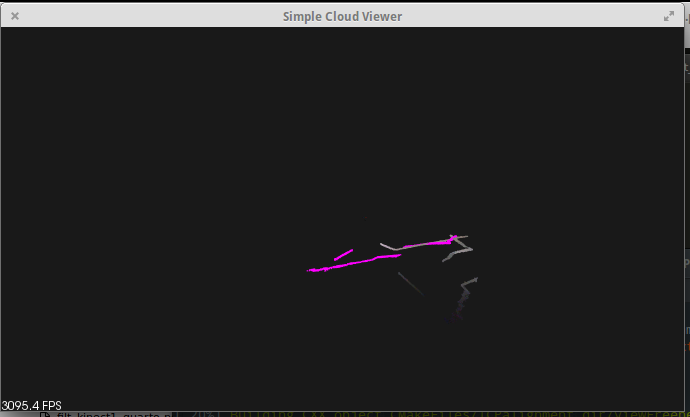
\includegraphics[width=70mm]{img/cozinha.png}
\caption{Resultado obtido após exercício 5 - cozinha}
\end{figure}


\begin{figure}[ht!]
\centering
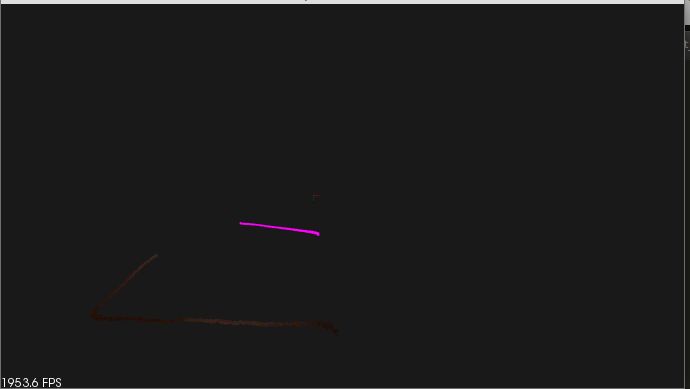
\includegraphics[width=70mm]{img/quarto.png}
\caption{Resultado obtido após exercício 5 - quarto}
\end{figure}

Como pode ser observado pelas imagens acima, os resultados não foram os melhores. Deve-se ao facto de termos capturado demasiados pontos e estes demorarem demasiado tempo a serem processados. Optamos por eliminar manualmente alguns desses e assim conseguirmos obter algum resultado.



\begin{thebibliography}{1} % 9



\bibitem{fsound}
Neves, A. J. R.; Dias, P. Slides teóricos Visão por Computador - Aula 7 (2016)


\bibitem{vtk}
OpenCV. \href{hhttp://docs.opencv.org/}{Opencv Documentation}. Web. 15 Outubro 2016. 




\end{thebibliography}

\end{document}
